\section{실험 및 결과}
\label{sec:experiments}

\revtwo{4장에서 정의한 입력ㆍ대조군ㆍ외부 검증 지표를 단계적으로 적용한다. 먼저 추가 학습 없이 가드 문장에 반응하는지를 진단하고, 이어 올바른 가드--행동 대응의 학습 가능성을 확인한다. 그다음 동일 목표의 정적 후보, 시간 유지ㆍ해제, 정지ㆍ차선 변경으로 적용 범위를 넓히고, 마지막에 별도 폐루프 환경에서 실행 차단의 역할을 분석한다. 각 실험은 확인 목적, 비교 방법, 결과 및 의미의 순서로 기술한다.}

실험 증거는 서로 직접 비교할 수 없는 세 묶음으로 나뉜다. 첫째, 추가 학습을 하지 않은 Alpamayo-R1의 단일 장면 사전 진단은 가드 문장에 대한 반응만 살펴본다. 둘째, 본 논문의 중심 증거인 Qwen3-VL-2B-Instruct 실험은 합성 정적ㆍ시간ㆍ다중 주행 과제에서 가드 기반 후보 선택의 학습 가능성을 평가한다. 셋째, 별도의 두 층 신경망과 1차원 운동 모델을 이용한 폐루프 실험은 실행 차단장치의 역할을 분석하는 보조 증거다. 서로 다른 모델과 과제를 하나의 성능 향상 계열이나 교차 모델 재현으로 해석하지 않는다.

Qwen 실험은 단순한 정지/진행 문제에서 시작한다. 이 과제는 장면만 보고도 답을 맞힐 수 있다는 한계가 있으므로, 이후에는 같은 장면과 같은 행동 목표를 유지하고 가드만 바꾸어 정답이 달라지는 쌍대 계약을 사용한다. 평가 범위는 정적 경계, 대기와 출발의 시간 조건, 정지와 차선 변경 순으로 넓힌다.

이 장에서 사용하는 "가드 준수 목표 완료율"은 실험에서 제시한 가드를 지키면서 CoC의 행동 목표까지 끝낸 예의 비율이다. 실제 도로의 모든 위험이 제거되었다는 뜻은 아니다. \revone{서로 다른 설정과 지표를 사용하는 실험의 역할을 먼저 구분할 수 있도록, 표~\ref{tab:suite}에 각 실험의 연구 질문ㆍ평가 설정, 핵심 비교, 주요 지표 및 증거의 범위를 함께 정리하였다. 행 사이의 절대 수치는 비교하지 않고 각 행의 핵심 비교 안에서 해석한다.}

\paragraph{평가 이름을 읽는 법.}
이후 모든 과제에서 \textbf{표준 평가}는 학습에 쓰지 않은 장면을 사용하되 문장 틀과 수치 범위는 학습 자료와 같은 평가를 뜻한다. \textbf{동일 의미 문장 변형 평가}는 제약의 뜻과 수치는 유지하고 문장 표현만 바꾼다. \textbf{미관측 수치 평가}는 문장 틀은 유지하되 학습에 없던 속도ㆍ거리ㆍ시간 값을 사용하며, 시간 과제에서는 이를 \textbf{미관측 시간값 평가}라 부른다. \textbf{복합 표현 변화 평가}는 경계값 등호, 부정ㆍ금지 표현, 절 순서 변경과 m--cm 단위 변환을 한 평가 집합에 함께 포함한다. 따라서 `동일 의미 문장 변형'은 말투 변화, `미관측 수치'는 새로운 숫자, `복합 표현 변화'는 여러 언어ㆍ단위 변화가 동시에 포함된 더 어려운 평가다. 표와 그림에서는 이를 각각 \textit{Standard evaluation}, \textit{Same-semantics paraphrase evaluation}, \textit{Unseen-value evaluation} 또는 \textit{Unseen-time-value evaluation}, \textit{Combined expression-shift evaluation}으로 표시한다. 표와 그림의 $\uparrow$는 클수록 좋고 $\downarrow$는 작을수록 좋다는 뜻이다. $a\pm b$는 세 번 반복한 결과의 평균 $a$와 표준편차 $b$이며, 모집단 또는 표본 표준편차 중 어느 것을 사용했는지는 각 표와 그림 설명에 명시한다.

\subsection{Alpamayo-R1 사전학습 상태 진단}

\paragraph{확인 목적.}
첫 실험의 질문은 간단하다. 학습하지 않은 가드 문장을 Alpamayo-R1의 CoC에 추가하면, 관찰한 장면에서 모델이 그 의미에 맞게 궤적을 바꾸는가? 이 실험은 차량 안전이나 Alpamayo-R1의 일반 성능을 평가하지 않는다. 별도의 가드 학습 없이 문장만 추가해도 되는지를 한 장면과 세 가지 행동 생성 초기값에서 먼저 확인하는 진단 실험이다.

\paragraph{비교 방법.}
장면과 기본 CoC는 그대로 두고 추가 문장만 바꾸었다. 하나는 기다리라는 가드이고, 다른 하나는 그와 반대로 진행을 허용하는 가드이다. 행동과 관계없는 문장도 비교에 사용하였다. 먼저 기본 CoC에 문장을 추가했을 때 2초 뒤 궤적이 얼마나 달라졌는지 계산하였다. 다음으로 서로 반대되는 두 가드가 만든 궤적의 차이를 계산하였다. 첫 번째 값은 모델이 추가 문장에 반응했는지를 보여준다. 두 번째 값은 단순히 문장이 들어온 것에 반응한 것이 아니라, 기다림과 진행이라는 반대 의미를 구별했는지를 보여준다.

\paragraph{결과.}
그림~\ref{fig:r1-diagnostic}에서 문장을 추가한 궤적은 기본 CoC의 궤적과 2초 뒤 0.263 m 차이가 났다. 즉, 모델은 추가 문장에 반응하였다. 그러나 기다리라는 가드와 진행을 허용하는 가드 사이의 차이는 0.008 m에 불과했다.

\paragraph{의미.}
관찰한 한 장면에서는 CoC에 문장을 추가하는 것 자체의 변화가 컸지만, 서로 반대되는 가드 사이의 의미 대비는 8 mm에 그쳤다. 이 변위는 준수 여부가 아니라 2초 뒤 궤적 차이를 재는 대리 지표이므로 Alpamayo-R1 전체의 의미 이해 실패로 일반화할 수 없다. 다만 이 진단만으로는 가드 문장을 넣는 것만으로 준수를 기대할 근거가 부족하다. 다음 실험에서는 별도의 작은 VLM에 가드와 올바른 행동의 관계를 직접 학습시킨다.

\begin{figure}[t]
\centering
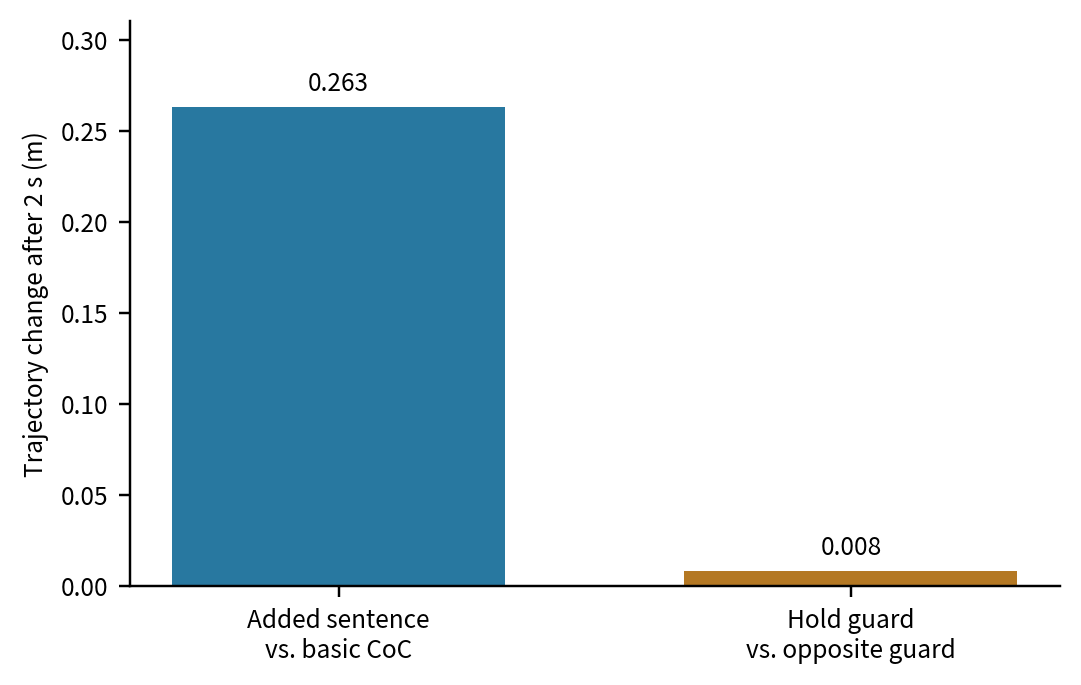
\includegraphics[width=0.94\columnwidth]{../latex-kiee-review-2022/figures/fig04_r1_diagnostic.png}
\bifigcaption{Alpamayo-R1 사전 진단. 첫 막대 0.263 m는 문장을 추가했을 때 기본 CoC와 달라진 정도이므로 `추가 문장에 대한 반응'을 나타낸다. 두 번째 막대 0.008 m는 대기 가드와 반대 가드의 차이이므로 `반대 의미의 구별'을 나타낸다. 두 번째 값이 매우 작아 이 한 장면만으로 의미에 맞는 가드 준수를 확인할 수 없다.}{Alpamayo-R1 pre-training diagnostic: sensitivity to added text is much larger than the trajectory contrast between opposite guard meanings.}
\label{fig:r1-diagnostic}
\end{figure}

\subsection{최소 가드-행동 학습과 초기 과제의 한계}

\paragraph{확인 목적.}
두 번째 실험은 작은 VLM이 "이 가드에서는 정지하고, 저 가드에서는 진행한다"는 대응을 학습할 수 있는지 확인한다. 동시에 정지와 진행만 구분하는 쉬운 문제가 가드의 효과를 실제보다 크게 보이게 할 수 있는지도 확인한다.

\paragraph{비교 방법.}
후보는 정지(STOP)와 진행(PROCEED) 두 가지로 만들었다. 첫 조건에서는 가드와 정답 행동을 올바르게 연결했다. 비교 조건에서는 같은 가드 문장을 사용하되 정답 행동과의 연결을 일부러 섞었다. 이 비교를 통해 모델이 단순히 문장을 받은 효과와 가드의 올바른 의미를 배운 효과를 구분한다. 평가는 학습에 사용하지 않은 장면과, 같은 뜻을 다른 문장으로 표현한 경우로 나누었다. 쉬운 과제에서는 학습량의 차이가 결과에 영향을 주지 않도록 기존 CoC와 CoC+Guard의 학습 횟수도 같게 맞추었다.

\paragraph{결과.}
표준 평가에서 올바른 제약--정답 대응을 학습한 조건의 후보 정확도는 0.990, 계약 쌍 정확도는 0.958이었다. 반면 제약--정답 대응을 교란한 통제군은 각각 0.719와 0.000이었다. 이는 올바른 제약--행동 관계를 학습하면 학습에 쓰지 않은 장면에서도 두 계약을 구별할 수 있음을 보여준다. 그러나 동일 의미 문장 변형 평가에서는 두 조건의 후보 정확도가 0.740과 0.745였고, 계약 쌍 정확도는 모두 0이었다. 즉, 표준 문장과 비슷한 입력에는 대응했지만 같은 뜻의 새로운 표현으로 일반화하지는 못했다.

또한 학습 자료가 충분한 쉬운 과제에서는 기존 CoC만 사용해도 후보 정확도 0.974와 계약 쌍 정확도 0.896에 도달했고, CoC+Guard는 1.000과 1.000이었다. 학습 횟수를 같게 맞춘 사후 비교에서는 두 조건 모두 두 지표가 1.000이었다.

\paragraph{의미.}
두 가지를 알 수 있다. 첫째, 작은 VLM은 가드와 행동의 관계를 학습할 수 있다. 둘째, 쉬운 정지/진행 문제에서는 가드가 없어도 장면만 보고 정답을 외울 수 있다. 이 경우 CoC+Guard의 높은 정확도가 정말 가드를 읽은 결과인지 분명하지 않다. 따라서 정적 실험은 모든 후보가 같은 CoC 목표를 달성하게 만들고, 시간 및 다중 주행 실험은 목표를 완료하는 경쟁 후보에 계속 정지하는 교착 후보를 더하여 가드 준수와 진행성을 함께 측정한다.

\begin{table*}[!t]
\color{reviewerone}
\centering
\bitablecaption{실험 전체의 읽기 안내. 각 행은 연구 질문과 평가 설정, 핵심 비교, 주요 지표 및 증거의 범위를 요약한다. 서로 다른 모델ㆍ과제의 행 사이 수치를 직접 성능 순위로 비교하지 않는다.}{Reading guide summarizing the question and setting, primary comparison, key endpoint, and evidential role of each experiment. Results are interpreted within, not across, rows.}
\label{tab:suite}
\scriptsize
\begin{tabularx}{\textwidth}{L{0.13\textwidth}L{0.22\textwidth}L{0.19\textwidth}L{0.18\textwidth}Y}
\toprule
Experiment & Question and evaluation setting & Primary comparison & Key endpoint & Evidential role \\
\midrule
R1 diagnostic & Does an untrained VLM distinguish opposite guards in one scene? & Basic CoC, hold guard, opposite guard & Trajectory change after 2 s & Text-sensitivity diagnostic; not a compliance test \\
Minimal learning & Can the model learn a correct guard--action mapping on held-out scenes and paraphrases? & Correct versus shuffled mapping & Candidate and paired accuracy & Initial learnability and easy-task limitation \\
Static candidates & Which equal-objective trajectory is admissible under a changed static bound? Standard/paraphrase/unseen-value tests & Basic CoC and four constraint representations & Violation, excess conservatism, paired accuracy & Static constraint-conditioned selection \\
Temporal condition & Does a changed hold duration switch the answer? Standard/paraphrase/unseen-time tests & Short- versus long-hold contracts & Violation, compliant completion, paired accuracy & Temporal release and numeric generalization \\
Stopping/lane change & Does the effect repeat across maneuvers? Standard and combined-shift hard cases & Proposed versus basic and shuffled conditions & Violation, compliant completion, paired accuracy & Multi-constraint and unit/expression robustness \\
Closed-loop auxiliary & Must a released contract be revoked when risk returns? Release-reversal episodes & State, CoC, monotone/dynamic contract, shield & Violation, collision, intervention cost & Reversible state update and runtime checking in a separate small network \\
\bottomrule
\end{tabularx}
\end{table*}

\subsection{동일 목표를 달성하는 정적 궤적 후보}

\paragraph{확인 목적.}
이 실험에서는 모든 후보가 "교차로를 통과한다"는 같은 목표를 달성한다. 따라서 모델은 목표 달성 여부만으로 정답을 고를 수 없다. 현재 가드가 어느 후보를 허용하는지 읽어야 한다.

\paragraph{비교 방법.}
두 후보 모두 교차로를 통과하지만 최대 속도, 장애물과의 최소거리, 진입 시점과 진행 속도가 다르다. 같은 장면에서 완화 계약은 더 빠른 후보를 허용하지만, 엄격 계약은 그 후보를 금지하고 더 신중한 후보를 허용한다. 표~\ref{tab:representations}의 기본 CoC, 제약 통합 CoC, 별도 자연어 제약, 제약--정답 대응 교란 및 논리식 제약을 비교하였다. 두 계약의 정답을 모두 맞혀야 하는 계약 쌍 정확도를 핵심 지표로 사용하였다.

이 정적 결과는 난수 초기값(seed) 42를 사용한 단일 학습 반복이다. 학습 자료는 96개 장면에서 만든 576개 예이고, 분리 평가는 24개 장면에 세 종류의 가드를 각각 쌍으로 적용한 144개 예다. 따라서 표~\ref{tab:static}의 작은 차이를 데이터 생성이나 학습 난수에 대해 안정적인 차이로 해석하지 않는다.

\begin{table*}[!t]
\centering
\bitablecaption{같은 행동 목표를 달성하는 정적 후보의 표준 평가. 후보 정확도와 계약 쌍 정확도는 높을수록 좋고, 가드 위반률과 과도한 보수 선택률은 낮을수록 좋다. 모든 조건의 목표 완료율이 1.000이므로 위반 감소가 목표 포기의 결과는 아니다. 모든 비율은 평가 예 144개를 분모로 한다.}{Standard evaluation of static candidates sharing the same behavioral goal. Accuracy and paired accuracy are higher-is-better; violation and excess conservatism are lower-is-better.}
\label{tab:static}
\footnotesize
\begin{tabularx}{\textwidth}{L{0.22\textwidth}ZZZZZ}
\toprule
Condition & Candidate accuracy & Guard violation rate $\downarrow$ & Excess-conservatism rate $\downarrow$ & Paired-contract accuracy $\uparrow$ & Goal completion rate \\
\midrule
Basic CoC (no constraint) & 0.500 & 0.250 & 0.250 & 0.000 & 1.000 \\
Constraint-integrated CoC (proposed) & \textbf{1.000} & \textbf{0.000} & \textbf{0.000} & \textbf{1.000} & 1.000 \\
Separate natural-language constraint & 0.993 & 0.007 & 0.000 & 0.986 & 1.000 \\
Shuffled constraint--target mapping & 0.465 & 0.188 & 0.347 & 0.153 & 1.000 \\
Logical-form constraint & \textbf{1.000} & \textbf{0.000} & \textbf{0.000} & \textbf{1.000} & 1.000 \\
\bottomrule
\end{tabularx}
\end{table*}

\paragraph{결과.}
표~\ref{tab:static}은 각 행이 무엇을 의미하는지 두 단계로 읽어야 한다. 먼저 마지막 열이 모두 1.000이므로 어느 조건도 교차로 통과 목표를 포기하지 않았다. 그다음 위반률과 계약 쌍 정확도를 보면, 제약 정보가 없는 기본 CoC는 선택의 0.250에서 가드를 위반했고 완화ㆍ엄격 계약을 모두 맞힌 장면은 없어 계약 쌍 정확도가 0.000이었다. 엄격 계약 72개만 분모로 한 원 저장 위반률은 0.500이지만, 다른 표와 정의를 맞추기 위해 여기서는 전체 144개 예 기준인 0.250을 사용하였다. 제약--정답 대응을 교란한 통제군의 계약 쌍 정확도도 0.153에 머물렀다.

반면 제약 통합 CoC와 논리식 제약은 위반률 0.000, 과도한 보수 선택률 0.000, 계약 쌍 정확도 1.000을 기록하였다. 별도 자연어 제약도 전체 예 기준 위반률 0.007과 계약 쌍 정확도 0.986을 기록하였다. 입력 형식이 같은 별도 자연어 제약과 제약--정답 대응 교란의 계약 쌍 정확도 차이 0.833은 제약 문장을 추가하는 것만으로는 부족하고, 올바른 제약--정답 대응을 학습해야 함을 보여준다.

동일 의미 문장 변형 평가의 후보/계약 쌍 정확도는 제약 통합 CoC 0.875/0.750, 별도 자연어 제약 0.924/0.847, 논리식 제약 1.000/1.000이었다. 미관측 수치 평가에서는 각각 1.000/1.000, 0.951/0.903, 0.924/0.847이었다. 여기서 슬래시 앞은 개별 문제의 후보 정확도, 뒤는 같은 장면의 두 계약을 모두 맞힌 계약 쌍 정확도다.

\paragraph{의미.}
제약 통합 CoC는 항상 정지하는 방법으로 위반을 피한 것이 아니다. 모든 후보가 목표를 완료했고, 그중 현재 계약이 허용하는 가장 진행도가 높은 후보를 골랐다. 따라서 이 결과는 모델이 실행 가드를 정적 후보 선택에 사용했음을 보여준다. 다만 정적 과제에서 논리식 제약이 높은 성능을 보였다는 이유만으로 논리 표현이 언제나 더 좋다고 결론 내릴 수는 없다. 다음 시간 과제에서는 다른 결과가 나타난다.

\subsection{정지-대기-해제-출발 시간 조건}

\paragraph{확인 목적.}
앞 실험은 속도나 거리처럼 한 시점의 기준을 다루었다. 이번 실험은 "얼마나 오래 기다려야 하며 언제 출발해도 되는가"라는 시간 조건도 모델이 배울 수 있는지 확인한다.

\paragraph{비교 방법.}
장면과 네 후보는 그대로 두고, 상충 구역이 비어 있는 것을 확인한 뒤 기다려야 하는 시간만 바꾸었다. 완화 계약은 짧게 기다린 뒤 출발하는 후보를 허용하고, 엄격 계약은 더 오래 기다린 후보만 허용한다. 후보는 조기 진입, 짧은 대기 후 진입, 긴 대기 후 진입과 계속 정지로 구성하였다. 각 난수 초기값에서 192개 장면으로 만든 384개 예를 학습하고, 48개 장면으로 만든 96개 계약 예를 평가하였다. 난수 초기값 42, 17, 123은 모델 초기화와 학습 순서뿐 아니라 합성 장면의 값과 후보 문자 배치도 함께 바꾼다. 따라서 세 반복은 전체 절차의 반복성을 보지만, 데이터를 고정한 채 최적화 분산만 분리하지는 않는다. 네 시점을 이어 붙인 연속 장면 영상에는 시각적 상태와 시간이 글자로 표시되고 후보 설명에는 후보 진입 시각이 적혀 있다. 저장한 어댑터를 재학습하지 않고 원본 영상, 정보가 없는 단색 영상, 실제와 다른 `상충 구역이 비기 시작한 시각'을 표시한 충돌 영상으로 각각 다시 평가하여 영상 정보의 기여를 분리하였다.

\begin{table*}[!t]
\centering
\bitablecaption{정지--대기--해제--출발 시간 과제의 표준 평가. 값은 세 난수 초기값 결과의 평균$\pm$모집단 표준편차다. 후보 정확도ㆍ계약 쌍 정확도와 가드 준수 목표 완료율은 높을수록 좋고, 가드 위반률과 교착률은 낮을수록 좋다.}{Standard temporal evaluation for stop--hold--release--go, reported as three-seed mean $\pm$ population standard deviation.}
\label{tab:temporal}
\footnotesize
\begin{tabularx}{\textwidth}{L{0.22\textwidth}ZZZZZ}
\toprule
Condition & Candidate accuracy & Guard violation rate $\downarrow$ & Deadlock rate $\downarrow$ & Guard-compliant goal completion rate $\uparrow$ & Paired-contract accuracy $\uparrow$ \\
\midrule
Basic CoC (no constraint) & $0.500\pm0.000$ & $0.319\pm0.052$ & $0.000\pm0.000$ & $0.681\pm0.052$ & $0.000\pm0.000$ \\
Constraint-integrated CoC (proposed) & $\mathbf{1.000\pm0.000}$ & $\mathbf{0.000\pm0.000}$ & $0.000\pm0.000$ & $\mathbf{1.000\pm0.000}$ & $\mathbf{1.000\pm0.000}$ \\
Separate natural-language constraint & $0.698\pm0.094$ & $0.191\pm0.136$ & $0.000\pm0.000$ & $0.809\pm0.136$ & $0.396\pm0.187$ \\
Shuffled constraint--target mapping & $0.510\pm0.015$ & $0.333\pm0.023$ & $0.000\pm0.000$ & $0.667\pm0.023$ & $0.021\pm0.029$ \\
Logical-form constraint & $0.538\pm0.027$ & $0.274\pm0.108$ & $0.000\pm0.000$ & $0.726\pm0.108$ & $0.076\pm0.055$ \\
\bottomrule
\end{tabularx}
\end{table*}

\paragraph{결과.}
표~\ref{tab:temporal}은 학습과 같은 문장 틀ㆍ시간값 범위를 사용한 표준 평가다. 제약 통합 CoC는 세 번의 반복 모두 가드 위반률 0.000, 가드 준수 목표 완료율 1.000, 계약 쌍 정확도 1.000을 기록하였다. 같은 연속 장면 영상에서 짧은 대기를 요구하면 짧은 대기 후보를, 긴 대기를 요구하면 긴 대기 후보를 골라 두 계약을 모두 맞힌 것이다. 반면 제약 정보가 없는 기본 CoC는 두 계약에 같은 입력을 받으므로 계약 쌍 정확도가 0.000이고 가드 위반률은 $0.319\pm0.052$였다. 별도 자연어 제약은 평균적으로 기본 CoC와 대응 교란 통제군보다 나았지만 난수 초기값에 따라 차이가 컸다. 대응 교란 통제군과 논리식 제약은 두 대기시간의 차이를 안정적으로 배우지 못했다.

\revone{위치만 바꾼 대비에서 제약 통합 CoC와 별도 자연어 제약의 후보 정확도는 각각 1.000과 0.698, 계약 쌍 정확도는 1.000과 0.396이며 가드 위반률은 0.000과 0.191이었다. 반면 같은 별도 필드 형식에서 올바른 대응을 학습한 조건과 대응 교란 조건의 계약 쌍 정확도는 0.396과 0.021이었다. 따라서 전자는 현재 모델에서 목표와 가드를 한 문맥에 배치한 위치ㆍ구획 효과를, 후자는 위치를 고정했을 때 올바른 가드--행동 대응의 효과를 보여준다. 정적 과제에서는 통합/별도 조건의 계약 쌍 정확도가 1.000/0.986으로 위치 효과가 작았으므로, 통합 위치의 이점은 모든 과제에 동일하게 일반화되지 않는다.}

그러나 그림~\ref{fig:temporal-pair}(a)처럼 제약 통합 CoC의 성능은 입력 변화에 따라 낮아졌다. 제약의 뜻과 수치는 같고 말투만 바꾼 \textbf{동일 의미 문장 변형 평가}에서는 후보 정확도 0.858, 가드 위반률 0.115, 가드 준수 목표 완료율 0.885, 계약 쌍 정확도 0.715였다. 문장 틀은 유지하고 학습에 없던 대기시간을 사용한 \textbf{미관측 시간값 평가}에서는 각각 0.635, 0.351, 0.649, 0.306이었다. 즉 문장 표현만 달라져도 성능이 일부 낮아졌고, 새로운 시간값에서는 더 크게 낮아졌다. 표준 평가의 완벽한 결과가 일반적인 시간 비교 규칙의 학습을 의미하지는 않는다.

저장한 세 난수 초기값의 제약 통합 CoC 어댑터를 다시 실행한 원본 영상 결과는 표~\ref{tab:temporal}과 모든 지표에서 정확히 일치하였다. 표~\ref{tab:image-ablation}의 각 셀은 `후보 정확도/계약 쌍 정확도' 순서다. 표준 시간 과제는 원본 1.000/1.000에서 단색 영상 0.670/0.403, 상충 구역이 비기 시작한 시각이 실제와 다른 충돌 영상 0.608/0.340으로 낮아졌다. 단색 영상과 시간 충돌 영상의 가드 위반률도 각각 0.288과 0.208이었다. 따라서 표준 과제의 완벽한 결과는 문장만 읽은 결과가 아니며 연속 장면 영상에 표시된 시간 정보에 의존한다. 반면 미관측 시간값 평가에서는 원본 후보 정확도부터 0.635에 그쳤고 영상 교란이 이를 일관되게 더 낮추지 않았다. 시간 충돌 영상은 문제의 관측 전제 자체를 바꾸므로 그 조건에서 우연히 낮아진 위반률이나 높아진 목표 완료율을 성능 향상으로 해석하지 않는다. 이는 새로운 시간값에서 시각 시간과 수치 관계를 안정적으로 결합하지 못했다는 추가 증거다.

\paragraph{의미.}
제약 통합 CoC는 표준 분포의 같은 장면에서도 제약이 요구하는 대기시간에 따라 출발 후보를 바꾸었다. 그러나 미관측 시간값 결과는 이 대응이 일반적인 시간 비교 규칙으로 충분히 일반화되지 않았음을 보여주므로 RQ4에는 부정적인 답을 준다. 기본 CoC는 두 계약에 동일한 입력을 받으므로 결정적 모델이 두 정답을 모두 구별할 수 없는 정보 부재 기준선이다. 따라서 기본 CoC의 후보 정확도 0.500과 계약 쌍 정확도 0.000을 제안법의 안전성 우월성으로 해석하지 않는다. 시간 과제에서 입력 형식이 같은 별도 자연어 제약과 제약--정답 대응 교란의 계약 쌍 정확도는 각각 0.396과 0.021이었다. 이 차이가 올바른 제약--정답 대응 학습의 더 직접적인 증거다. 반면 제약 통합 CoC와 대응 교란 조건의 차이에는 입력 위치의 효과도 포함된다. 논리식 제약의 낮은 결과도 논리식 자체가 자연어보다 나쁘다는 뜻은 아니다. 두 표현을 공정하게 비교하려면 논리 문법을 별도로 학습시킨 뒤 다시 평가해야 한다.

\subsection{정지ㆍ차선 변경과 복합 표현 변화}

\paragraph{확인 목적.}
앞 실험의 성공이 대기시간 문제에만 나타난 결과일 수 있다. 이를 확인하기 위해 정지와 차선 변경으로 행동을 넓혔다. 또한 같은 가드를 다른 문장이나 처음 보는 수치로 표현해도 모델이 조건을 지키는지 확인하였다.

\paragraph{비교 방법.}
정지 과제에서는 정지선 위치, 최대 감속도와 최대 가가속도를 가드로 사용하였다. 차선 변경 과제에서는 최소 차량 간격과 중단 후 재시도 조건을 사용하였다. 192개 장면마다 완화 계약과 엄격 계약을 하나씩 적용하여 384개 학습 예를 만들었다. 표준 평가, 동일 의미 문장 변형 평가와 미관측 수치 평가는 각각 48개 장면, 즉 96개 계약 문제로 구성하였다. 별도의 \textbf{복합 표현 변화 평가}에는 (1) 측정값이 기준값과 정확히 같은 경계 등호, (2) 부정ㆍ금지 문장, (3) 조건절 순서 변경, (4) 같은 값을 m 대신 cm로 적는 단위 변환을 함께 넣었다. 따라서 이 평가는 네 요인 중 하나의 원인을 분리하는 요인별 실험이 아니라, 여러 표현 변화가 섞인 강건성 시험이다. 저장 어댑터는 원본, 단색 및 반대 행동 종류의 영상에서도 다시 평가하였다.

\revone{표준 평가의 반복적인 1.000이 난이도 부족을 가릴 수 있으므로, 위 복합 표현 변화 평가를 \textbf{hard-case 평가}로 명시하여 행동별로도 재집계하였다. 정지 hard-case는 정지선, 감속도 및 가가속도 세 제약을 동시에 적용하고, 완화 계약의 두 수치 상한을 빠른 후보의 측정값과 정확히 같게 두어 판정 여유가 0인 경계 등호를 포함한다. 차선 변경 hard-case도 완화 계약의 최소 간격을 빠른 후보의 측정값과 같게 두고, 간격 미달 시 중단ㆍ재시도하는 조건을 함께 적용한다. 각 난수 초기값의 48개 장면은 정지와 차선 변경을 24개씩 포함하며, 장면마다 완화ㆍ엄격 계약을 적용한 총 96개 문제다.}

\begin{table*}[!t]
\centering
\bitablecaption{정지ㆍ차선 변경 과제의 표준 평가와 복합 표현 변화 평가. 값은 세 난수 초기값 결과의 평균$\pm$표본 표준편차다. `복합 표현 변화'에는 경계 등호, 부정ㆍ금지, 절 순서 변경 및 m--cm 단위 변환이 함께 포함된다. 단위 정규화 행은 저장 어댑터의 재평가 결과다.}{Standard and combined-expression-shift evaluations for stopping and lane change, including re-evaluation of saved adapters after deterministic unit normalization; values are three-seed mean $\pm$ sample standard deviation.}
\label{tab:maneuver}
\footnotesize
\begin{tabularx}{\textwidth}{L{0.15\textwidth}L{0.22\textwidth}ZZZZ}
\toprule
Evaluation & Condition & Candidate accuracy & Guard violation rate $\downarrow$ & Guard-compliant goal completion rate $\uparrow$ & Paired-contract accuracy $\uparrow$ \\
\midrule
Standard evaluation & Basic CoC (no constraint) & $0.500\pm0.000$ & $0.292\pm0.072$ & $0.708\pm0.072$ & $0.000\pm0.000$ \\
 & Constraint-integrated CoC (proposed) & $\mathbf{1.000\pm0.000}$ & $\mathbf{0.000\pm0.000}$ & $\mathbf{1.000\pm0.000}$ & $\mathbf{1.000\pm0.000}$ \\
 & Shuffled constraint--target mapping & $0.503\pm0.006$ & $0.267\pm0.039$ & $0.733\pm0.039$ & $0.028\pm0.032$ \\
\midrule
Combined expression-shift evaluation & Basic CoC (no constraint) & $0.500\pm0.000$ & $0.302\pm0.065$ & $0.698\pm0.065$ & $0.000\pm0.000$ \\
 & Constraint-integrated CoC (proposed) & $\mathbf{0.948\pm0.063}$ & $\mathbf{0.010\pm0.010}$ & $\mathbf{0.990\pm0.010}$ & $\mathbf{0.896\pm0.127}$ \\
 & \revone{Proposed + unit normalization} & \revone{$\mathbf{0.958\pm0.072}$} & \revone{$\mathbf{0.000\pm0.000}$} & \revone{$\mathbf{1.000\pm0.000}$} & \revone{$\mathbf{0.917\pm0.144}$} \\
 & Shuffled constraint--target mapping & $0.535\pm0.079$ & $0.260\pm0.018$ & $0.740\pm0.018$ & $0.090\pm0.139$ \\
\midrule
\revone{Hard-case by maneuver} & \revone{Proposed: stopping} & \revone{$0.979\pm0.021$} & \revone{$0.021\pm0.021$} & \revone{$0.979\pm0.021$} & \revone{$0.958\pm0.042$} \\
 & \revone{Proposed: lane change} & \revone{$0.917\pm0.144$} & \revone{$0.000\pm0.000$} & \revone{$1.000\pm0.000$} & \revone{$0.833\pm0.289$} \\
\bottomrule
\end{tabularx}
\end{table*}

\paragraph{결과.}
표~\ref{tab:maneuver}의 위쪽 세 행은 표준 평가, 아래쪽 세 행은 복합 표현 변화 평가다. 표준 평가에서 제약 통합 CoC는 정지와 차선 변경 모두 가드 위반률 0.000, 가드 준수 목표 완료율 1.000, 계약 쌍 정확도 1.000을 기록하였다. 즉, 두 행동에서 목표를 완료하면서 완화ㆍ엄격 계약에 따라 정답 후보를 정확히 바꾸었다. 기본 CoC보다 평균 위반률은 0.292 낮았다. 난수 초기값을 단위로 다시 뽑아 계산한 95\% 구간은 [0.250, 0.375]였다. 같은 입력 형식을 사용한 제약--정답 대응 교란 통제군보다 계약 쌍 정확도는 0.972 높았고 해당 구간은 [0.938, 1.000]이었다. 따라서 이 차이는 단순한 제약 문장 추가보다 올바른 제약--정답 대응 학습의 효과를 직접 보여준다. 다만 반복이 세 번뿐이고 각 난수 초기값에서 데이터도 함께 바뀌므로 이 구간은 확정적인 통계 결론이 아니라 전체 절차에서 관찰된 범위를 살펴보는 참고값이다.

복합 표현 변화 평가에서 제약 통합 CoC의 가드 위반률은 $0.010\pm0.010$, 계약 쌍 정확도는 $0.896\pm0.127$로 표준 평가보다 낮아졌다. 오답 15개는 모두 같은 거리를 m 대신 cm로 표현한 문장에서 관찰되었다. 난수 초기값 42의 오답 12개는 가드를 위반하지는 않았지만 필요 이상으로 느린 차선 변경 후보를 선택한 경우였다. 나머지 3개는 난수 초기값 17과 123에서 감속도 또는 가가속도 상한을 넘은 정지 후보를 선택한 경우였다. 부정 표현, 조건절 순서 변경과 m 단위 경계값만 포함한 예에서는 오답이 없었다. 그러나 여러 변화가 한 평가 집합에 함께 있으므로 이 관찰만으로 단위 변환이 유일한 원인이라고 확정할 수는 없다.

\revone{단위 정규화 효과를 분리하기 위해 저장된 세 어댑터와 동일한 288개 hard-case 문제를 다시 사용하고, 72개 cm 문장의 수치와 단위만 동등한 m 표현으로 결정적으로 변환한 뒤 재평가하였다. 장면, 후보, 정답, 나머지 문장 및 모델 가중치는 바꾸지 않았다. cm 부분집합의 정답은 57/72(0.792)에서 60/72(0.833)로 3건 회복되었고 회귀한 정답은 없었다. 이에 따라 전체 후보 정확도는 0.948에서 0.958, 계약 쌍 정확도는 0.896에서 0.917로 높아졌으며, 세 건의 안전하지 않은 정지 선택이 모두 교정되어 가드 위반률은 0.010에서 0.000으로 낮아졌다. 그러나 난수 초기값 42의 과도하게 보수적인 차선 변경 오답 12건은 남았다. 비-cm 입력의 예측은 하나도 변하지 않았다. 따라서 단위 정규화는 수치 안전 오류를 제거하는 실용적인 전처리였지만, 복합 문장에 대한 보수적 선택까지 해결하지는 못했다.}

\revone{행동별 hard-case에서 제약 통합 CoC의 후보/계약 쌍 정확도는 정지 0.979/0.958, 차선 변경 0.917/0.833이었다. 정지의 가드 위반률은 0.021이었고 차선 변경의 가드 위반률은 0이었지만, 차선 변경에서는 가드를 지키면서도 더 느린 후보를 고른 과도한 보수 선택 때문에 계약 쌍 정확도가 더 낮았다. 이 하락은 표준 평가의 1.000을 일반적인 난제 해결 성능으로 해석할 수 없고, 동시 제약ㆍ경계 등호ㆍ표현 변화가 모델 차이를 드러내는 데 필요함을 보여준다.}

다중 주행의 표준 평가와 미관측 수치 평가는 단색 영상과 반대 행동 영상에서도 세 난수 초기값 모두 후보 정확도와 계약 쌍 정확도 1.000을 유지하였다. 복합 표현 변화 평가의 원본/단색/반대 행동 영상은 각각 후보 정확도 0.948/0.906/0.948, 계약 쌍 정확도 0.896/0.813/0.896이었다. 이 과제의 영상은 행동 종류별 고정 도식이고 후보 물리량과 행동 종류가 문장에 직접 적혀 있으므로, 높은 표준ㆍ미관측 수치 결과는 시각적 근거화가 아니라 주로 문장 기반 제약 후보 선택의 증거다.

\begin{table*}[!t]
\centering
\bitablecaption{저장 어댑터의 영상 절제 재평가. 각 셀은 `후보 정확도/계약 쌍 정확도' 순서의 세 난수 초기값 평균이다. 단색 영상은 시각 정보를 제거한다. 충돌 영상은 시간 과제에서 상충 구역이 비기 시작한 시각을 실제와 다르게 표시하고, 다중 주행 과제에서는 문장과 반대되는 행동 도식을 제시한다. 충돌 영상은 입력 전제를 바꾸므로 강건성 향상이 아니라 영상 의존성 진단으로만 읽는다.}{Image-ablation re-evaluation of saved adapters. Each cell reports candidate accuracy/paired-contract accuracy averaged over three seeds.}
\label{tab:image-ablation}
\footnotesize
\begin{tabular}{llccc}
\toprule
Task & Evaluation & Original image & Blank image & Conflicting image \\
\midrule
Temporal & Standard evaluation & 1.000/1.000 & 0.670/0.403 & 0.608/0.340 \\
 & Unseen-time-value evaluation & 0.635/0.306 & 0.691/0.382 & 0.705/0.410 \\
Stopping and lane change & Standard evaluation & 1.000/1.000 & 1.000/1.000 & 1.000/1.000 \\
 & Combined expression-shift evaluation & 0.948/0.896 & 0.906/0.813 & 0.948/0.896 \\
\bottomrule
\end{tabular}
\end{table*}

\paragraph{의미.}
제약을 CoC 안에 함께 제시하는 효과는 대기시간뿐 아니라 정지와 차선 변경에서도 나타났다. 그러나 복합 표현 변화 평가에서는 오류가 남았다. 오답이 cm 표현에 집중되었더라도 여러 변화가 함께 포함된 평가이므로 모든 오류의 원인이 단위 변환이라고 확정할 수는 없다. 후속 실험에서는 단위, 부정 표현, 조건 순서와 경계값을 한 번에 하나씩만 바꾸어 원인을 분리해야 한다.

\begin{figure*}[!t]
\centering
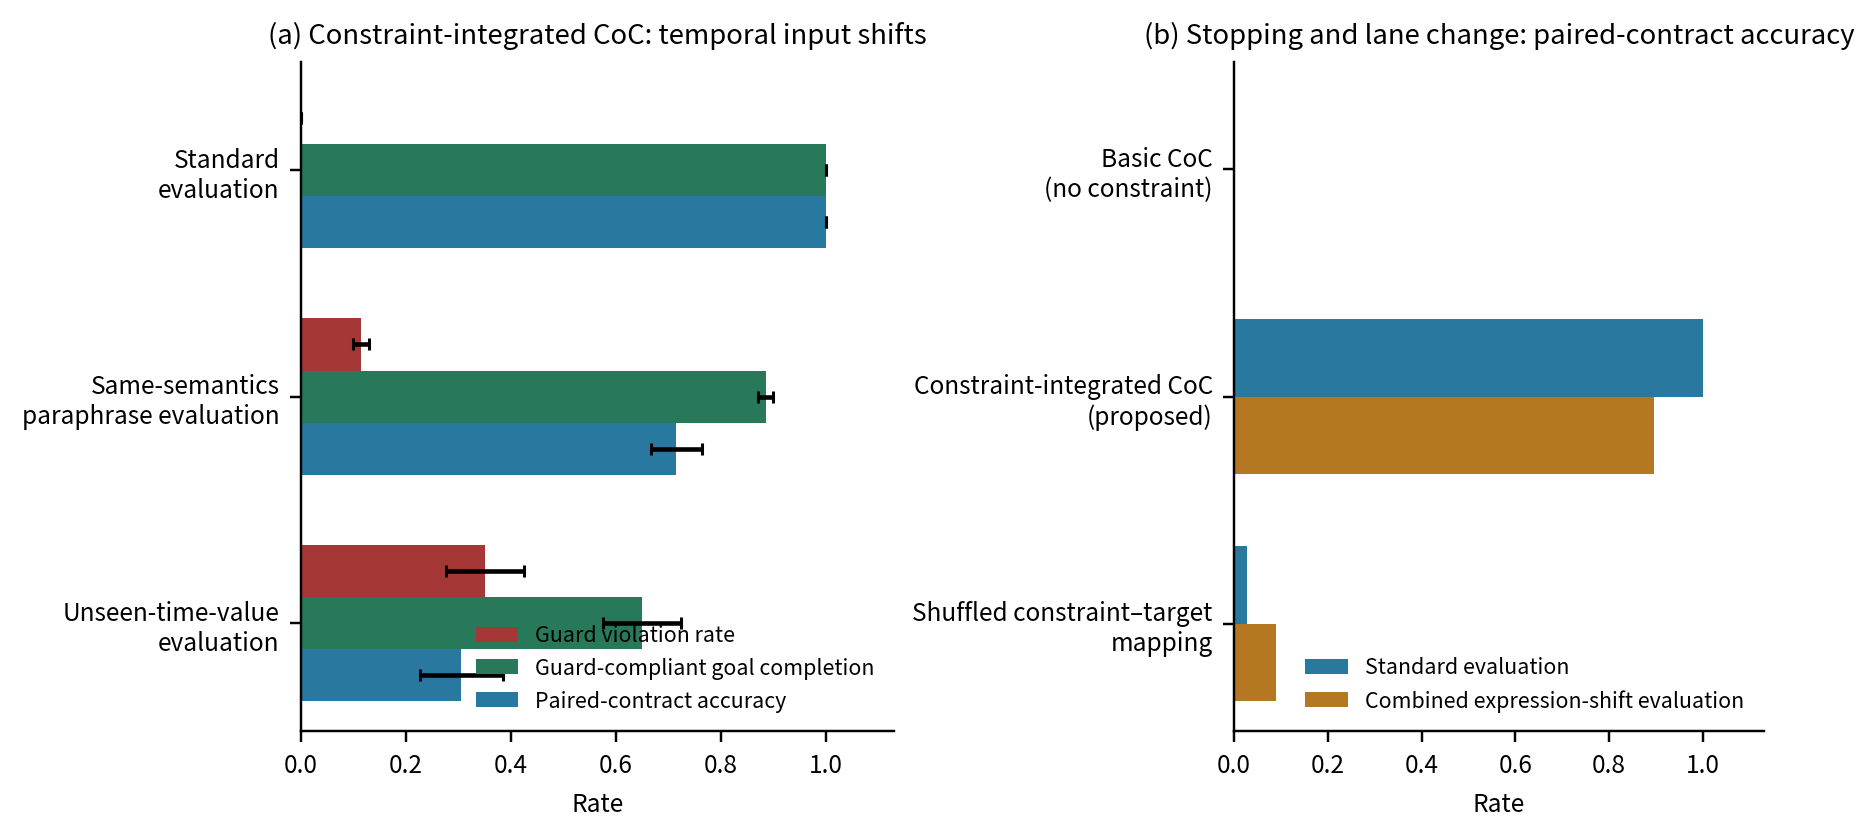
\includegraphics[width=0.98\textwidth]{../latex-kiee-review-2022/figures/fig05_temporal_pair.png}
\bifigcaption{입력 변화에 따른 성능. (a)는 제약 통합 CoC의 시간 과제를 비교한다. 빨간색 가드 위반률은 낮을수록, 초록색 가드 준수 목표 완료율과 파란색 계약 쌍 정확도는 높을수록 좋다. 표준 평가에서는 위반률 0.000, 나머지 두 지표 1.000이지만 동일 의미 문장 변형 평가에서 낮아지고, 미관측 시간값 평가에서 가장 크게 낮아진다. (b)는 정지ㆍ차선 변경 과제의 계약 쌍 정확도다. 파란색은 표준 평가, 주황색은 경계ㆍ부정ㆍ순서ㆍ단위 변화가 함께 든 복합 표현 변화 평가다. 기본 CoC와 대응 교란 통제군은 낮고 제약 통합 CoC만 두 평가에서 높은 값을 유지한다. (a)의 오차 막대는 모집단 표준편차이며 (b)의 표 값은 표본 표준편차를 사용한다.}{Performance under input shifts. Panel (a) shows temporal degradation from standard to paraphrased and unseen-time evaluations; panel (b) compares paired-contract accuracy under standard and combined expression shifts.}
\label{fig:temporal-pair}
\end{figure*}

\subsection{폐루프 보조 실험}

\paragraph{확인 목적.}
앞의 실험은 VLM이 미리 주어진 후보를 한 번 선택하는 문제였다. 마지막 실험은 선택 뒤에도 상황이 계속 바뀌는 경우를 살펴본다. 학습된 계약만 사용할 때와, 실행 중 위험한 명령을 막는 차단 장치를 함께 사용할 때를 비교한다. 이 실험은 작은 신경망과 단순한 운동 모델을 사용한 보조 분석이며, 앞의 VLM 결과나 실제 차량과 직접 비교하지 않는다.

\paragraph{비교 방법.}
두 층 신경망과 1차원 운동학으로 만든 소규모 폐루프 환경을 사용하였다. 폐루프란 모델이 한 번만 답하는 것이 아니라, 매 시점의 상태를 다시 받아 다음 행동을 계속 정하는 환경을 뜻한다. \textbf{상태 전용(State only)}은 수치 상태만, \textbf{상태+CoC(State + CoC)}는 상태와 행동 목표를 입력한다. \textbf{동적 계약(Dynamic contract)}은 현재 위험에 따라 대기와 출발 허용을 양방향으로 갱신한다. \textbf{단조 단계 계약(Monotone-stage contract)}은 한 번 출발을 허용하면 위험이 다시 생겨도 대기로 돌아가지 않는다. \textbf{계약+차단장치(Contract + shield)}는 동적 계약에 더해 실행 직전 위험한 명령을 막는다. 그림의 \textit{Delayed} 조건은 계약 정보가 실제 상태보다 0.4초 늦게 도착한 경우다.

\revone{해제 후 재위험 episode의 핵심 상태전이는 $\mathrm{HOLD}\rightarrow\mathrm{RELEASED}\rightarrow\mathrm{HOLD}$이다. $t=0$에 출발이 허용되더라도 $t=0.8$에 다른 차량이 다시 나타나면 기존 허용을 취소하고 대기 가드를 재활성화해야 한다. 동적 계약은 현재 위험을 반영하여 이 역전이를 표현하지만, 단조 단계 계약은 $\mathrm{RELEASED}$에 고정되어 현재 허용 범위를 잘못 나타낸다. 따라서 이 비교는 계약에 해제 조건만 두는 것으로 충분한지, 해제 이후에도 센서 상태에 따라 가드를 되살리는 reversible update가 필요한지를 평가한다.}

평가는 두 상황으로 나누었다. 첫째, 학습 자료에 정지, 대기, 출발 등 모든 주행 단계가 충분히 들어 있는 상황이다. 둘째, 출발이 허용된 뒤 다른 차량이 다시 나타나므로 다시 정지해야 하지만 학습에서는 보지 못한 "해제 후 위험 재등장" 상황이다. 앞으로 1.2초의 모든 상황을 미리 아는 조건도 넣었지만, 이는 실제 방법이 아니라 도달 가능한 가장 좋은 결과를 보기 위한 참고값이다.

\revone{차단장치의 비용은 episode당 평균 개입 횟수뿐 아니라 동일한 300개 episode bank에서 차단장치가 없는 계약 조건 대비 평균 진행거리와 평균 절대 가가속도의 변화로 측정하였다. 진행거리 감소는 효율 손실의 대리 지표이고 가가속도 증가는 승차감 비용의 대리 지표다. 이 평가는 개별 개입이 반드시 필요했는지를 판정하는 독립 oracle을 포함하지 않으므로, 개입 횟수를 개별 불필요 개입률로 해석하지 않는다.}

\begin{figure*}[!t]
\centering
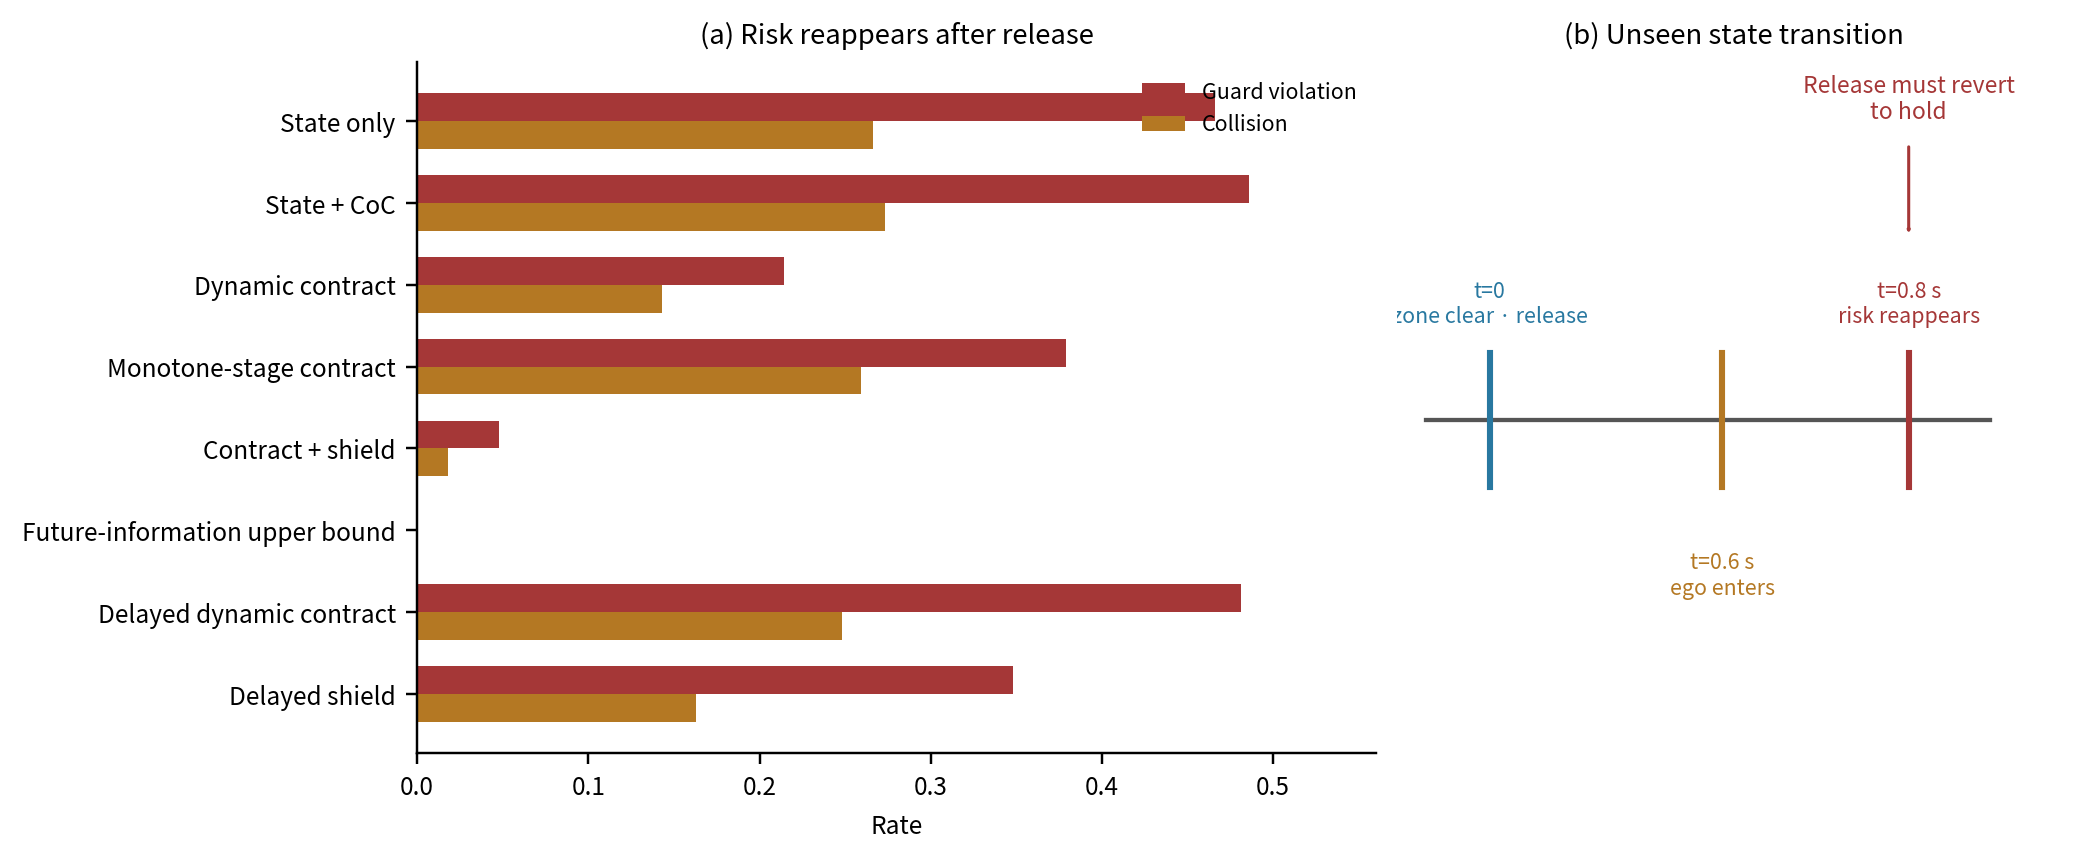
\includegraphics[width=0.98\textwidth]{../latex-kiee-review-2022/figures/fig06_release_reversal.png}
\bifigcaption{폐루프 보조 실험. (a)의 빨간 막대는 가드 위반률, 주황 막대는 충돌률이며 둘 다 낮을수록 좋다. 출발 허용 뒤 위험이 다시 나타날 때 상태 전용과 상태+CoC는 약 0.47--0.49의 위반률을 보이고, 최신 동적 계약은 0.214, 계약+차단장치는 0.048로 낮춘다. 계약 정보가 0.4초 늦으면 다시 악화된다. (b)는 $t=0$ 출발 허용, $t=0.6$ ego 진입, $t=0.8$ 위험 재등장 순서와 다시 대기로 돌아가야 하는 이유를 보여준다. 미래정보 상한은 앞 상황을 완벽히 안다는 비현실적 참고값이다.}{Auxiliary closed-loop experiment showing lower-is-better guard-violation and collision rates when risk reappears after release, together with the event timeline.}
\label{fig:release-reversal}
\end{figure*}

\paragraph{결과.}
먼저 모든 주행 단계를 학습한 상황을 보았다. 정지 후 대기로 넘어가는 예 1,404개를 학습 자료에 추가하자 상태 전용, 상태+CoC, 동적 계약과 단조 단계 계약 모두 300회 평가에서 정지 구간에 너무 일찍 들어가지 않았다. 학습 분포 밖 상황의 가드 위반률도 상태 전용 2.6\%, 상태+CoC 1.4\%, 동적 계약, 단조 단계 계약과 계약+차단장치는 모두 0\%였다. 이 경우 차단장치는 위반률을 더 낮추지 못했지만 주행할 때마다 평균 2.539회 개입했다. 이미 학습으로 해결된 상황에서는 차단장치가 불필요하게 작동할 수 있음을 뜻한다.

그러나 그림~\ref{fig:release-reversal}의 해제 후 재위험 상황에서는 결과가 달랐다. 가드 위반률은 상태 전용 46.6\%, 상태+CoC 48.6\%, 동적 계약 21.4\%, 단조 단계 계약 37.9\%, 계약+차단장치 4.8\%였다. 동적 계약은 현재 위험 상태를 알려 주어 위반을 줄였고, 차단장치는 위험한 행동을 실행 직전에 막아 위반을 더 줄였다. 충돌률도 같은 순서로 26.6\%, 27.3\%, 14.3\%, 25.9\%, 1.8\%였다.

\revone{같은 해제 후 재위험 bank에서 동적 계약은 단조 단계 계약보다 가드 위반률을 16.5\%p(37.9\%에서 21.4\%), 충돌률을 11.6\%p(25.9\%에서 14.3\%) 낮췄다. 두 조건은 모두 목표 완료율 100\%였으므로 이 차이는 영구 정지로 얻은 결과가 아니다. 단조 상태가 과거의 출발 허용을 유지하는 동안 동적 상태는 재등장한 위험에 맞추어 대기 가드를 다시 제공한다는 차이가 성능 격차와 일치한다. 다만 동적 계약도 위반을 없애지는 못했으므로 reversible update는 필요한 정보 갱신이지 그 자체로 실행 안전 보장은 아니다.}

모든 조건의 목표 완료율은 100\%였으므로 낮은 위반률이 단순히 차량을 계속 세운 결과는 아니었다. 앞으로의 상황을 완벽히 아는 비현실적 조건만 위반과 충돌이 모두 0\%였다. 또한 계약 정보가 실제 상황보다 0.4초 늦게 도착하면 동적 계약의 위반률은 48.1\%, 계약+차단장치는 34.8\%로 증가하였다. 올바른 계약도 늦게 전달되면 효과가 크게 줄어든다는 뜻이다.

\begin{table*}[!t]
\color{reviewerone}
\centering
\bitablecaption{차단장치의 안전 이득과 개입 비용. 값은 세 난수 초기값 평균이며, 변화량은 차단장치가 없는 대응 계약 대비 차단장치 조건의 차이다. 모든 조건의 목표 완료율은 1.000이었다.}{Safety benefit and intervention cost of the shield. Deltas compare each shielded condition with its corresponding unshielded contract condition; all completion rates were 1.000.}
\label{tab:shield-cost}
\footnotesize
\begin{tabularx}{\textwidth}{L{0.18\textwidth}L{0.18\textwidth}ZZZZ}
\toprule
Evaluation bank & Comparison & Violation/collision change & Interventions per episode & Progress change (m) & Mean absolute jerk change \\
\midrule
Phase-complete ID & Phase contract $\rightarrow$ shield & $0.000/0.000$ & 1.269 & $-0.076$ & $+0.065$ \\
Phase-complete OOD & Phase contract $\rightarrow$ shield & $0.000/0.000$ & 2.539 & $-0.078$ & $+0.040$ \\
Release-reversal & Dynamic contract $\rightarrow$ shield & $-0.166/-0.125$ & 9.935 & $-0.030$ & $+0.306$ \\
\bottomrule
\end{tabularx}
\end{table*}

\revone{표~\ref{tab:shield-cost}에서 모든 주행 단계를 학습한 phase-complete bank의 ID와 OOD 조건은 차단장치 없이도 위반과 충돌이 0이었다. 차단장치는 추가적인 이진 안전 이득 없이 episode당 각각 1.269회와 2.539회 개입했고, 평균 진행거리를 0.076 m와 0.078 m 줄이며 평균 절대 가가속도를 0.065와 0.040 높였다. 반면 해제 후 재위험 bank에서는 episode당 9.935회의 개입과 함께 동적 계약 대비 위반률을 0.166, 충돌률을 0.125 낮추었고, 진행거리 0.030 m 감소와 평균 절대 가가속도 0.306 증가가 동반되었다. 따라서 차단장치는 미관측 재위험에서 안전 이득을 제공했지만, 이미 이진 안전지표가 포화된 bank에서는 이득 없이 보수적 개입 비용만 발생했다.}

\paragraph{의미.}
이 소규모 폐루프 환경에서는 충분한 성공 시연이 있을 때 문장에 적히지 않은 일부 제약도 행동 예에서 학습되었다. 이때 차단장치를 항상 사용하면 위반률을 더 낮추지 못하면서 개입만 늘어날 수 있었다. 그러나 학습하지 않은 위험이 다시 나타나면 동적 계약만으로는 위반을 모두 막지 못했다. 최신 상태를 사용하는 차단장치를 함께 사용했을 때 위반과 충돌이 가장 크게 줄었고, 그 효과도 계약 정보가 늦으면 감소했다. 이는 별도 미시 환경에서 실행 검사와 정보 최신성의 역할을 보여주는 결과이며, Qwen VLM이나 실제 차량에서 같은 감소율을 기대할 근거는 아니다.

\revone{그러므로 실제 시스템 관점의 비교는 위반ㆍ충돌 감소만으로 끝나지 않고 개입 빈도, 진행 손실 및 승차감 대리 지표를 함께 보고해야 한다. 본 실험은 개입 비용을 정량화했지만 개별 개입의 필요성을 판정하는 독립 oracle은 없으므로 intervention precision은 후속 평가 과제로 남는다.}
